\documentclass[../../main.tex]{subfiles}

    \lstset{basicstyle=\small,
      showstringspaces=false,
      commentstyle=\color{black},
      keywordstyle=\color{blue}
    }

    \graphicspath{{images/et/}{../../images/et/}}


    \begin{document}
    \subsection{Software TinyK22} \label{et_software_tiny}
    Dieses Kapitel beschreibt die Software, welche auf dem Mikrocontroller TinyK22 implementiert ist. Diese Software kommuniziert mit mit dem Pi und steuert die nötigen Sensoren und aktoren an. Die Schnittstelle zum Pi ist in Kapitel \ref{interface_pi_tiny} beschrieben. Weiteres Angaben zu den Sensoren und Aktoren und deren elektrische Verbindungen sind in Kapitel \ref{et_verbindungen} und \ref{et_Komponenten}.\\
    Die Software auf dem Mikrocontroller wird gemäss \ref{tab:et_mc_softwarekonzept} in verschiedene Module unterteilt. Jedes Modul initialisiert jeweils alle nötigen Komponenten. Die Komponenten initialisieren jeweils die nötigen Hardware Schnittstellen und allfällige Sub-Komponenten.\\

    \begin{table}[H]
        \centering
        \begin{tabular}{|l|p{12cm}|}
        \hline
        \textbf{Modulname} & \textbf{Beschreibung}    \\ \hline
        com   & Kommunikation mit dem pi                                                                                 \\ \hline
        cube  & Würfelerkennung mit Ansteuerung des TOF Sensors über I2C                                                 \\ \hline
        drive & Ansteuerung des Antriebmotors mit Regelung der Geschwindigkeit mittels dem Feedback vom Quadraturencoder \\ \hline
        crane & Ansteuerung des Motors für den Schwenker mit Positionsregelung mittels dem Feedback vom Quadraturencoder \\ \hline
        \end{tabular}
        \caption{Module Software TinyK22}
        \label{tab:et_mc_softwarekonzept}
    \end{table}


    In Abbildung \ref{fig:et_mc_softwarekonzept} ist die Aufteilung veranschaulicht. Mit grün sind jeweisl die einzelnen Module gekennzeichnet. Die Module benutzen jeweils ihre Komponenten abwärts bis zum Zugriff auf die Hardware. In Abbildung \ref{fig:et_mc_softwarekonzept} gelb gekennzeichnet repräsentiert die Komponenten, welche auf die Hardware des Mikrocontrollers zugreifen. Orange kennzeichnet die Komponenten, welche als Schnittstellen zwischen dem Hardwarezugriff und der Logik dienen. Diese Bereiten Informationen der Hardware auf in ein Format, dass die Logik gut verarbeiten kann. Die Logik ist in den rot gekennzeichneten Komponenten implementiert. Diese verarbeitet die Daten und trifft Entscheidungen.
    In Abbildung \ref{fig:et_mc_softwarekonzept} aus Übersichtsgründen nicht ersichtlich ist, dass alle module auf das com modul zugreifen können um mit dem Pi zu kommunizieren. Dabei benützen die Module die Komponenten comPi, comAck und comLog.\\

    \begin{figure}[H]
        \centering
        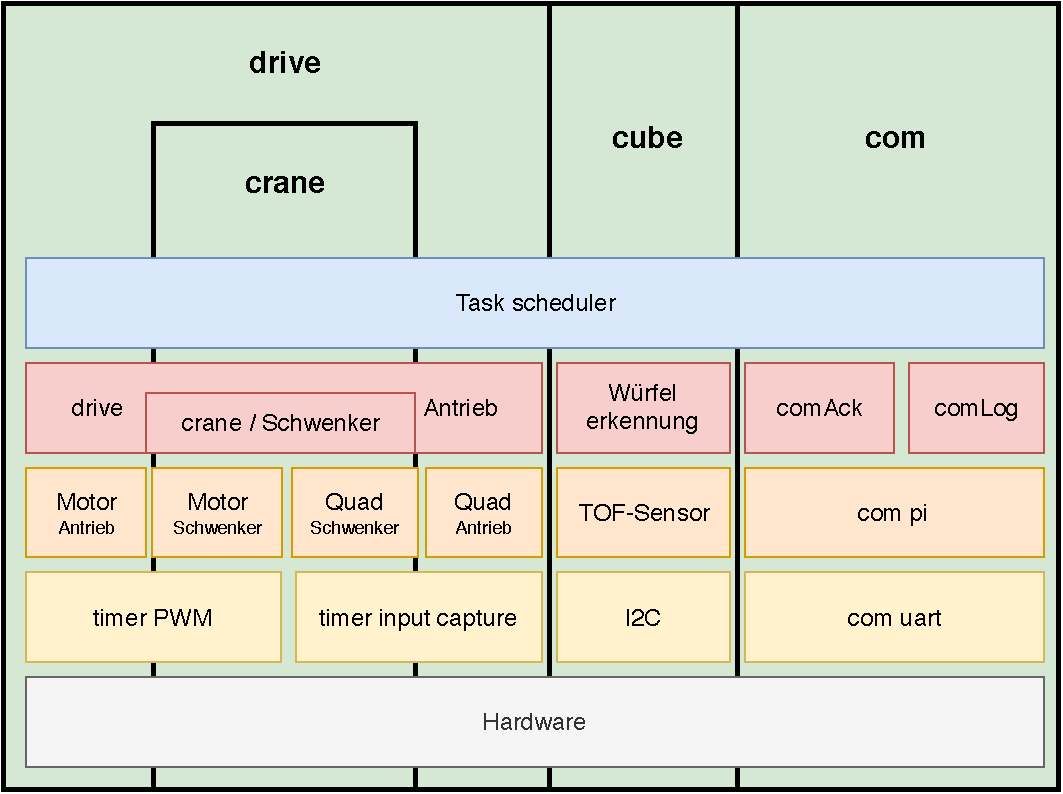
\includegraphics[width=0.8\textwidth]{../../images/et/et_mc_softwarekonzept.pdf}
        \caption {Modulaufteilung TinyK22}
        \label{fig:et_mc_softwarekonzept}
    \end{figure}

    \textbf{Task Scheudler}\\
    Für jedes Modul gibt es eine Taskfunktion, die während des Betriebs in einem Task Scheduler Loop periodisch aufgerufen wird. Auf die Benutzung eines Betriebssysteme wurde in diesem Projekt verzichtet. Der es gibt also keine Prioritäten oder Time-Slicing für die Tasks. Abbildung \ref{fig:et_task_scheudler} veranschaulicht das Prinzip der Implementation für einen Task. Wichtig dabei zu beachten ist, dass mit dieser Variante die vorgegebenen Zeitintervalle nicht exakt und je nach Auslastung variieren. Da die Tasks aber ohnehin nicht stark zeitkritisch sind funktioniert dies trotzdem. Alle Zeitkritischen Aufgaben werden über Interrupts behandelt.

    \begin{figure}[H]
        \centering
        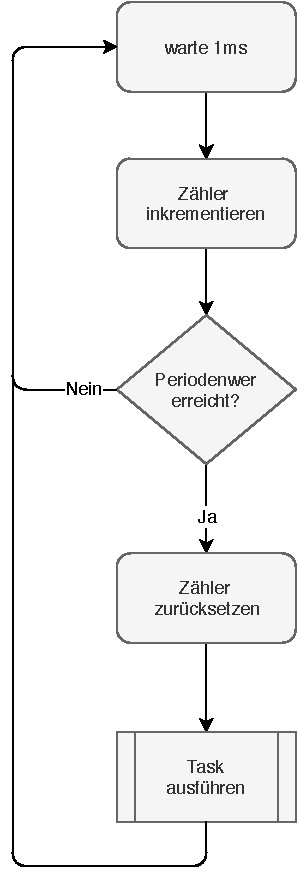
\includegraphics[width=0.3\textwidth]{../../images/et/et_task_scheudler.pdf}
        \caption {Flussdiagramm Task Scheudler}
        \label{fig:et_task_scheudler}
    \end{figure}

    \subsubsection{Modul com} \label{et_software_tiny_com}
    Das Modul com ist in verschiedene Komponente unterteilt. In Tabelle \ref{tab:et_mc_com} sind die verschiedenen Komponenten und deren Funktion aufgelistet. Die Komponente uart regelt den Zugriff auf die Hardware der UART-Schnittstelle und die Komponente pi verarbeitet die Frames allgemein. Die übrigen Komponenten benutzen für ihre Aufgabe jeweils diese beiden Komponenten als Basis.

    \begin{table}[H]
        \centering
        \begin{tabular}{|l|p{12cm}|}
        \hline
        \textbf{Komponente} & \textbf{Beschreibung}    \\ \hline
        uart  & regelt den Zugriff auf die Hardware Schnittstelle und Interrupts \\ & hat einen Ringbuffer implementiert, in dem die Empfangenen Daten zwischengespeichert werden.\\ \hline
        pi    & hat einen Task implementiert in dem periodisch der Ringbuffer der Komponente uart überprüft und wenn nötig ausgelesen wird \\ & bei einem vollständig Empfangenen Frame wird das entsprechende Modul informiert und der Empfangene Wert übergeben \\ \hline
        comAck & speichert und verwaltet alle ausstehenden acknowledge Meldungen \\ \hline
        comLog & Alle Module können mit den Funktionen und Makros dieser Komponente geordnete Log Meldungen an das Pi Schicken \\ & mit einem durch eine Präprozessor-Anweisung einstellbaren logLevel kann die Menge an nicht wichtigem Informationsaustausch reduziert werden \\ \hline
        \end{tabular}
        \caption{Komponente Modul pi}
        \label{tab:et_mc_com}
    \end{table}

    Im folgenden sind die Komponenten des Moduls uart jeweils beschrieben.\\

    \textbf{uart}\\
    Diese Komponente ermöglicht anderen Komponenten einen einfachen Zugriff auf die UART Schnittstelle. Es wird ein Sende- und Empfangs-Ringbuffer verwaltet. Diese Komponente Stellt funktionen zur verfügung um einzelne Zeichen oder ganze Zeilen in den Sende-Ringbuffer zu schreiben oder vom Empfangs-Ringbuffer zu lesen.\\
    Für das Empfangen und Senden einzelnder Zeichen ist in dieser Komponente ein Interrupt Handler für die UART Schnittstelle implementiert.\\

    \textbf{pi}\\
    Diese Komponente Stellt funktionen zur verfügung um Strings, signed Int oder unsigned Int für ein bestimmtes frame Topic zu versenden. Auch kann beim Senden einen Acknowledge-Handler angegeben werden (genauere Angaben dazu im Abschnitt comAck). Desweiteren können Module hier einen FrameLineHandler registrieren. In diesem wird ein bestimmtes Topic und eine Funktionszeiger angegeben. Wenn ein Frame mit dem angegeben Topic empfangen wird, ruft die Komponente pi diese angegeben Funktion auf und übergibt den empfangen Wert. Damit kann das Modul auf gewünschte Topics informiert werden.\\
    Die Funktion piDoWork() wird als Task periodisch aufgerufen und überprüft den Empfangs-Ringbuffer auf neue Frames. Ist ein solches angekommen wird das entsprechende Topic identifiziert und das entsprechende Modul über den Handler informiert. Abbildung \ref{fig:et_com_pi_handler} veranschaulicht den Ablauf der Kommunikation zwischen einem Modul und der Komponente pi.

    
    \begin{figure}[H]
        \centering
        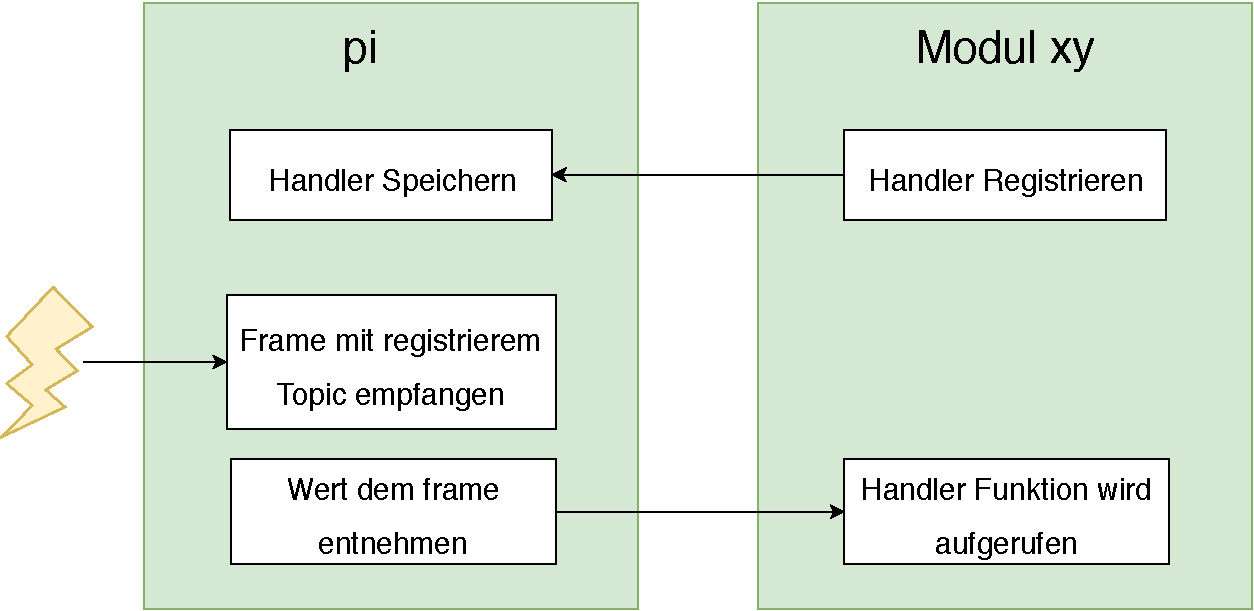
\includegraphics[width=0.8\textwidth]{../../images/et/et_com_pi_handler.pdf}
        \caption {Ablauf mit Frame Handler}
        \label{fig:et_com_pi_handler}
    \end{figure}

    \textbf{comAck}\\
    Damit ein Modul sicherstellen kann, dass seine verschickten Nachrichten beim Pi angekommen sind, kann dafür ein ackHandler registriert werden. Beim Senden einer Nachricht kann dieser dann als Ausstehend markiert werden. \\
    Die Funktion ackCheckQueue() wird dann als Task periodisch aufgerufen. Diese überprüft welche Acknowledge noch ausstehend sind und Informiert das Modul über den ackHandler wenn ein Acknowledge zu lange nicht empfangen wird.\\
    Um festzustellen welche Acknowledge empfangen werden, registriert die Komponente comAck einen FrameLineHandler bei der Komponente pi gemäss vorherigem Abschnitt.\\

    \subsubsection{Modul cube} \label{et_software_tiny_cube}
    Das Modul cube benutzt den TOF-Sensor über die I2C Schnittstelle um zu erkenne ob der Würfel neben dem Zug erkannt wurde. Sobald der Würfel erkennt wurde wird das Pi informiert.\\
    Die Komponenten beinhalten die Implementation für das I2C Protokoll und die nötige Kommunikation mit dem TOF-Sensor. Diese Komponenten werden dann von der Komponente cubeDetection benutzt und die Daten ausgewertet und davon eine Entscheidung getroffen.

    \begin{table}[H]
        \centering
        \begin{tabular}{|l|p{12cm}|}
        \hline
        \textbf{Komponente} & \textbf{Beschreibung}    \\ \hline
        I2C     & Implementation des I2C Protokolls und den Zugriff auf die Hardware der I2C Schnittstelle \\ \hline
        VL53L0X & Initialisierung und Kommunikation für den TOF-Sensor \\ & benutzt die Komponente I2C \\ \hline
        cubeDetection & Wertet die Daten des TOF-Sensor aus und entscheidet wann der Würfel erkannt wurde und meldet dies dem pi \\ \hline
        \end{tabular}
        \caption{Komponente Modul cube}
        \label{tab:et_mc_cube}
    \end{table}

    \textbf{I2C}\\
    Für die Implementation des I2C Protokolls wird eine Komponente aus dem Unterricht an der HSLU verwendet. Diese initialisiert die Hardware Schnittstelle und stellt sicher dass das I2C Protokoll korrekt umgesetzt wird. Sie stell Funktionen zur verfügung um in ein Register auf dem Slave zu schreiben und von einem Register von dem Slave zu lesen.\\

    \textbf{VL53L0X}\\
    Dies ist eine Bibliothek für den TOF-Sensor VL53L0X. Sie wird vom Hersteller Pololu zur verfügung gestellt, ist aber nur für Arduino Systeme verfügbar. Für diese Projekt wurde die Blibliothek angepasst, damit der Zugriff auf die I2C Schnittstelle über die Funktionen der im vorhergehenden Abschnitt beschriebenen Komponente erfolgt. \\
    Diese Komponente stellt Funktionen zur verfügung um den Sensor zu initialisieren und danach bei Bedarf den aktuellen Messwert auszulesen.\\

    \textbf{cubeDetection}\\
    Diese Komponente wertet die Daten des des TOF-Sensors aus und entscheidet wann der Würfel erkannt wurde. Die Funktion cubeDoWork() wird periodisch als Task aufgerufen. Dort wird der TOF-Sensor ausgelesen und der gemessene Wert mit einem Schwellwert verglichen. Die Ermittlung dieses Schwellwertes ist in Kapitel \ref{et_sensoren} beschrieben.\\
    Das Modul kann drei Zustände einnehmen. Diese sind ''notFound'', ''finding'' und ''found''. Der Initialzustand ist ''notFound''.\\
    Sobald der Schwellwert bei einer Messung unterschritten wurde, wird der Zustand in ''finding'' geändert und es werden noch 20 weitere Messungen durchgeführt und mit dem Schwellwert verglichen. Von diesen 20 Messungen müssen mindestens 90\% den Schwellwert ebenfalls unterschreiten um in den Zustand ''found'' zu wechseln. Durch diese Verifizierung können einzelne Fehlmessungen gefiltert werden. Werden die 90\% bei der Verifizierung nicht erreicht wird noch überprüft ob mindestens 50\% den Schwellwert unterschritten haben. Ist dies der Fall wird sofort eine neuer Verifizierung gestartet und der Zustand bleibt auf ''finding''. Ist dies nicht der Fall geht das Modul wieder in den Zustand ''notFound''.\\
    Abbildung \ref{fig:et_cube_detection_proc} veranschaulicht den Ablauf der Würfelerkennung.

    \begin{figure}[H]
        \centering
        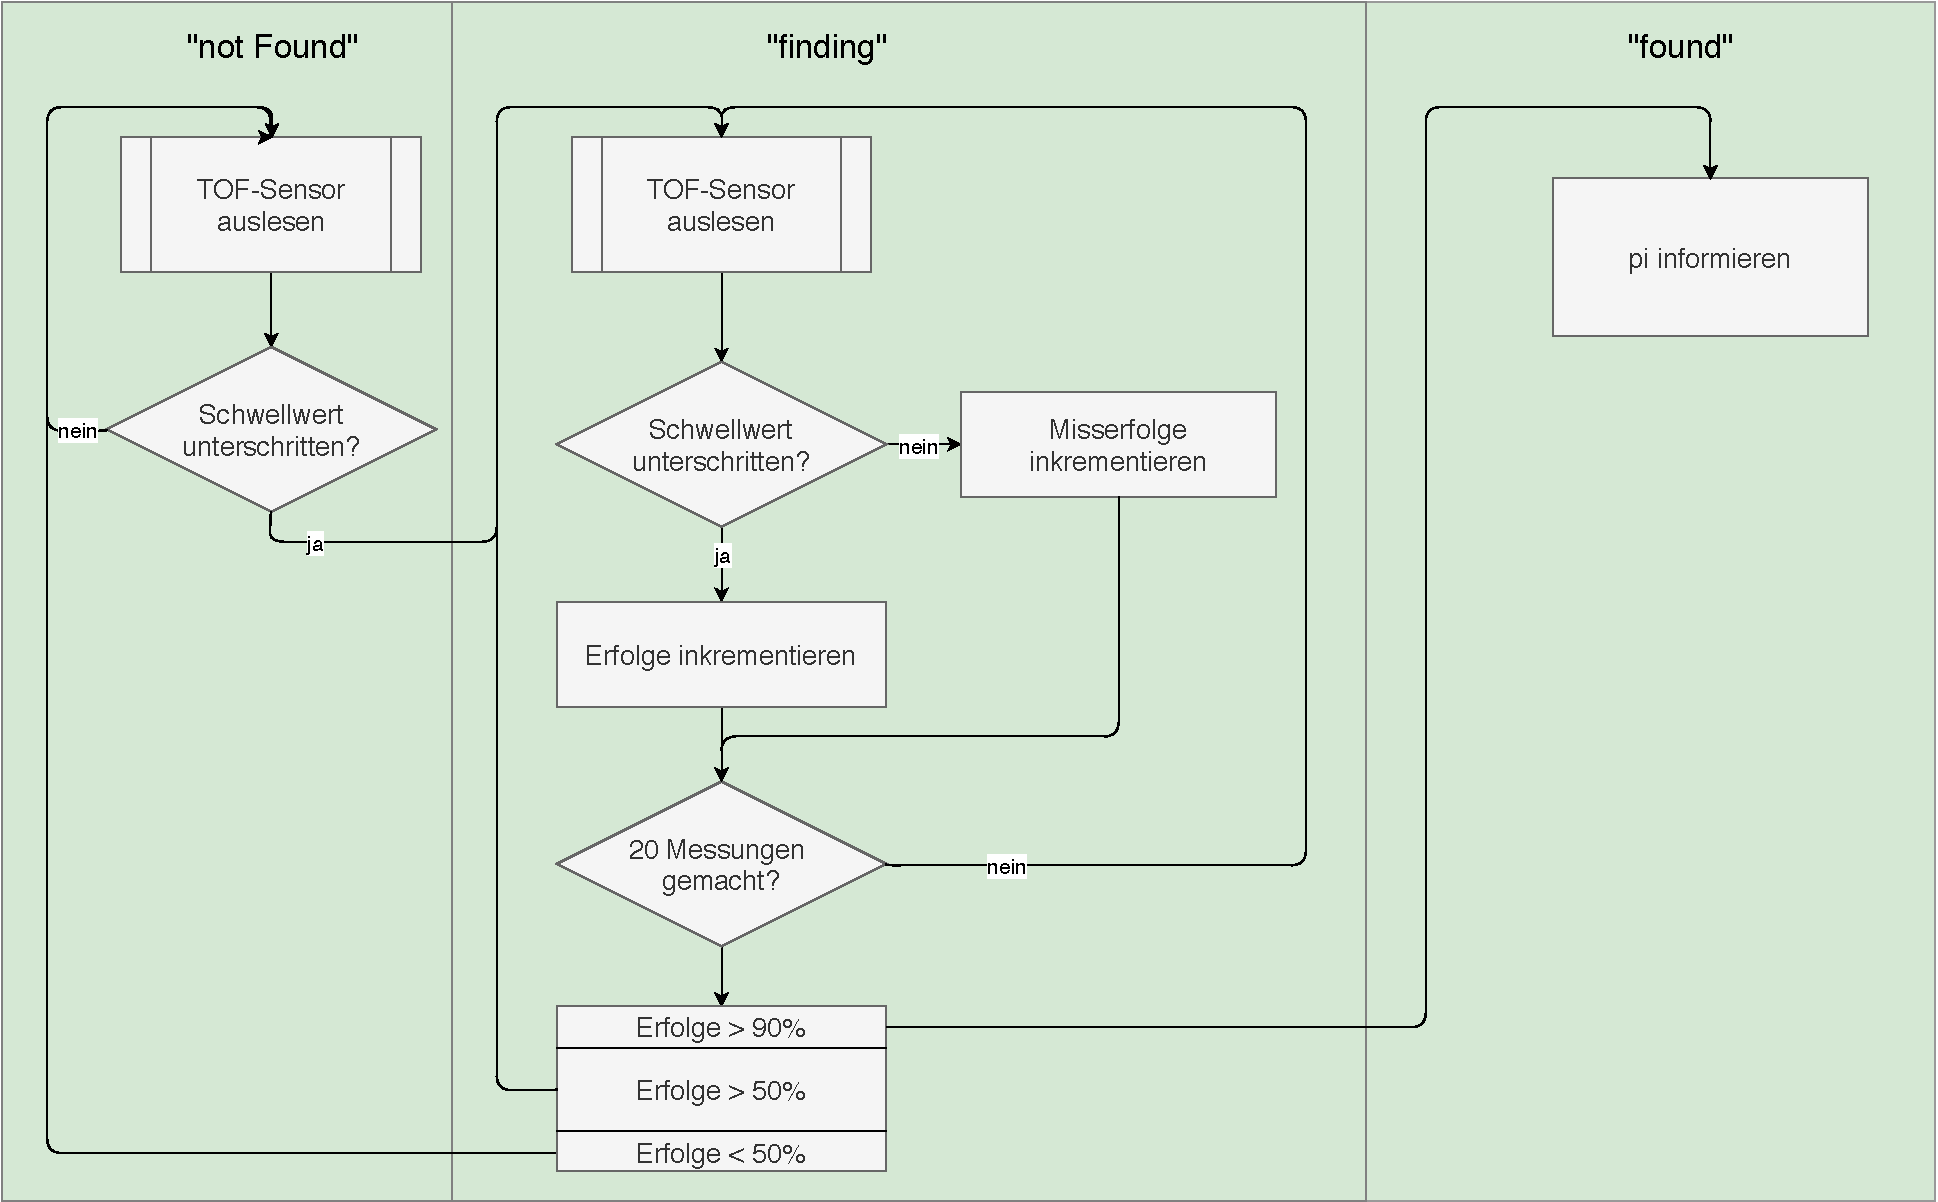
\includegraphics[width=1.0\textwidth]{../../images/et/et_cube_detection_proc.pdf}
        \caption {Ablauf für die Würfelerkennung}
        \label{fig:et_cube_detection_proc}
    \end{figure}

    \subsubsection{Modul drive} \label{et_sw_modul_drive}
    Für den Antrieb ist das Modul drive zuständig. Hier wird der Antriebsmotor angesteuert, die wahre Geschwindigkeit über den Quadraturencoder bestimmt und mit diesem Feedback dann die Geschwindigkeit durch eine Regelung stabilisiert.\\

    \begin{table}[H]
        \centering
        \begin{tabular}{|l|p{12cm}|}
        \hline
        \textbf{Komponente} & \textbf{Beschreibung}    \\ \hline
        motor  & Ansteuerung des PWM für den Motor über ein Hardware Timer-Modul \\ \hline
        quad   & Zählt die Impulse des Quadraturencoders und bestimmt die wahre Geschwindigkeit des Zuges \\ \hline
        drive  & wertet die Geschwindigkeit der Komponente quad aus und setzt anhande dieses Feedbacks die Ansteuerung des Motors mit der Komponente motor \\ \hline
        \end{tabular}
        \caption{Komponente Modul drive}
        \label{tab:et_mc_drive}
    \end{table}

    \textbf{motor}\\
    Die Komponente motor setzt den Hardware Timer des Mikrocontrollers gemäss den Vorgaben. Dabei kann mit der Funktion ''motor\_A\_SetPwm()'' der Duty-Cycle des PWMs eingestellt werden. Dabei kann ein Wert zwischen  $-100'000$ und $100'000$ übergeben werden. Das Vorzeichen bestimmt dabei die Richtung. ($-$ entspricht rückwärts fahren)\\

    \textbf{quad}\\
    Mit der Komponente quad wird die wahre Geschwindigkeit des Zuges bestimmt. Dazu werden die Impulse des des Quadraturencoders über eine bestimmte Zeit gezählt und daraus die Geschwindigkeit bestimmt. Um die Zeit des Messintervalls möglichst genau zu haben wird dafür ein Timer eingesetzt. Dieser überläuft jeweils nach $10 ms$. Beim Überlauf dieses Timers werden die Anzahl Impulse gespeichert und der Zähler wieder auf null zurückgesetzt.\\
    Die Geschwindigkeit des Zuges kann dann mit der Formel \ref{eq:et_v_zug} auf Seite \pageref{eq:et_v_zug} in der Software bestimmt werden.

    \textbf{drive}\\
    In dieser Komponente ist die Taskfunktion driveToWork(). Diese wird periodisch aufgerufen. Dabei wird die wahre Geschwindigkeit bestimmt und mit der Soll-Geschwindigkeit verglichen. Damit die wahre Geschwindigkeit möglichst gut der Soll-Geschwindigkeit entspricht, ist in dieser Taskfunktion ein PID-Regler implementiert. Die Stellgrösse dieses Reglers steuert mittels der Komponente motor den Antriebmotors an. Abbildung \ref{fig:et_drive_pid} zeigt das allgemeine Funktionsprinzip eines PID-Reglers. 
    \nocite{PIDcontroller}

    \begin{figure}[H]
        \centering
        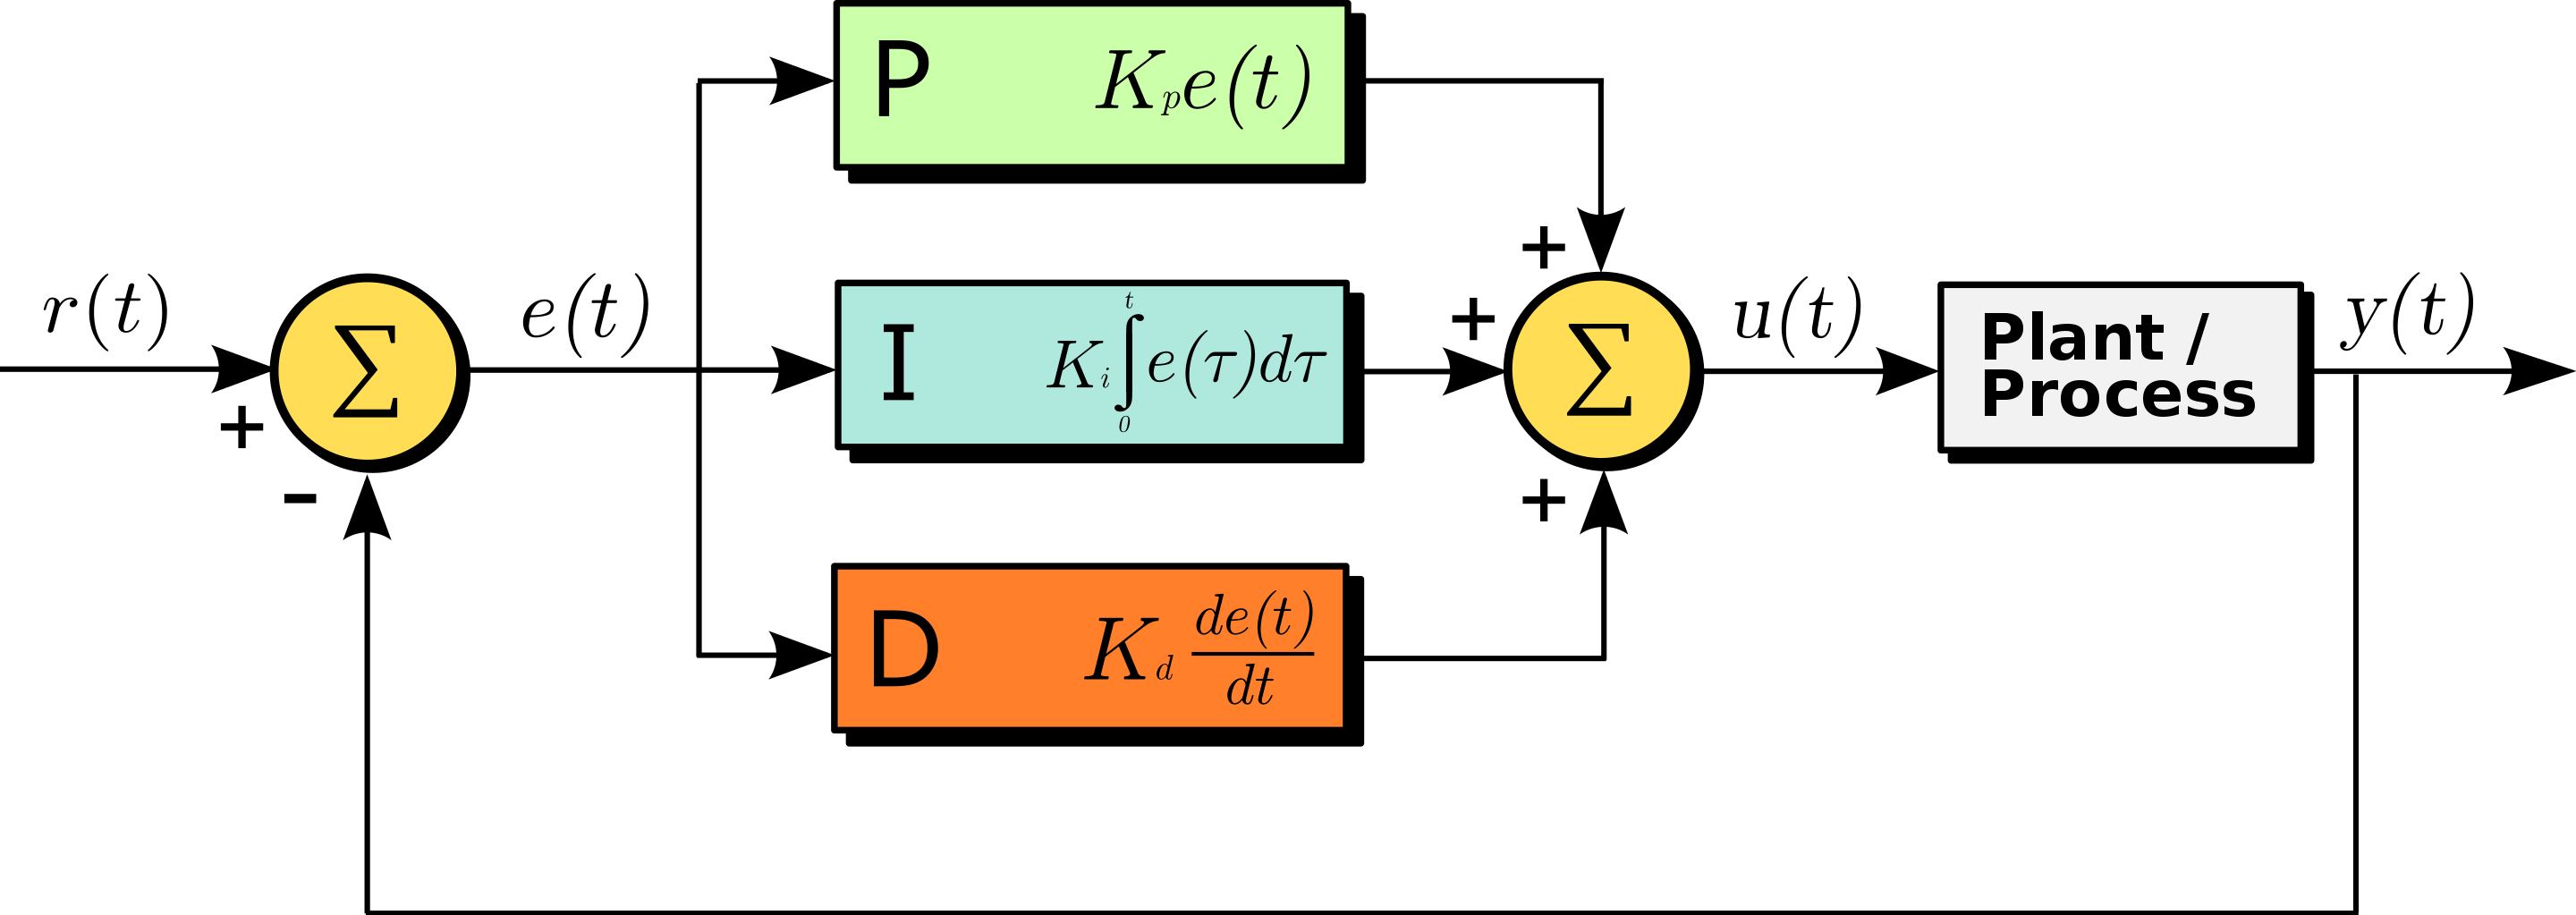
\includegraphics[width=0.6\textwidth]{../../images/et/et_wiki_PID_en.png}
        \caption {Allgemeines Prinzip eines PID-Reglers\\Quelle: Wikipedia.org - PID controller}
        \label{fig:et_drive_pid}
    \end{figure}

    Auch begrenzt das Modul drive die Beschleunigung des Zuges indem die Soll-Geschwindigkeit nicht direkt als von der Vorgabe übernommen wird, sondern mit einer Konstanten Steigung nachgeführt wird bis die Vorgabe-Geschwindigkeit erreicht ist. Damit beschleunigt der Zug mit höchstens einem Millimeter pro Sekunde pro Mikrosekunde.\\

    \subsubsection{Modul crane}
    Das Modul crane steuert den Motor für den Schwenker an. Es sorgt dafür, dass der Würfel auf Befehl vom Pi aufgenommen wird. Es besteht aus nur einer Komponente crane. In dieser Komponente wird der Schwenker Motor angetrieben bis am Quadraturencoder eine Vorgegebene Anzahl Impulse erfasst wurden. Diese Anzahl Impulse wir gemäss Kapitel \ref{et_sensoren} und Abbildung \ref{fig:et_schwenker_messung} auf Seite \pageref{fig:et_schwenker_messung} ermittelt.
    \end{document}